% presentation
\documentclass[comptress]{beamer}

\usepackage{mtex,fancyvrb,booktabs}
\usepackage{tikz,pgfplots}


\author{R. Hielscher}

\title{Denoising EBSD Data}

\institute{Faculty of Mathematics,\\
	Chemnitz University of Technology, Germany}

\date{{\bf{\color{red}M}TEX} Workshop 2017}


\author[R. Hielscher]{Ralf Hielscher}

\begin{document}

\frame[plain]{\titlepage}

%\begin{frame}

%  \tableofcontents

%\end{frame}



\begin{frame}[fragile]
  \frametitle{Noise in EBSD Data}

  \begin{columns}
    \begin{column}{8.3cm}
      \begin{overlayarea}{\textwidth}{\textheight}
      \begin{lstlisting}[style=input]
ebsd = loadEBSD('someData.txt')
\end{lstlisting}
\begin{onlyenv}<1>
        \begin{lstlisting}[style=output]
ebsd = /+EBSD+/ (show methods, plot)

 Phase  Orientations  Mineral  Symmetry
     0         30200       Al      m-3m

 Properties: ci, fit, iq, sem, x, y
 Scan unit : um
\end{lstlisting}
\end{onlyenv}
\pause
\vspace{-0.33cm}
      \begin{lstlisting}[style=input]
[grains,m2m] = calcGrains(ebsd)
plot(grains.boundary)
\end{lstlisting}
\begin{onlyenv}<2>
          \begin{lstlisting}[style=output]
grains = grain2d (show methods, plot)

 Phase  Grains  Pixels  Mineral  Symmetry  Crystal reference frame
     0      25   30200       Al      m-3m

 Properties: GOS, meanRotation
\end{lstlisting}
\end{onlyenv}
\pause
\vspace{-0.33cm}
\begin{lstlisting}[style=input]
plot(ebsd,m2m.angle)
\end{lstlisting}
\pause
\vspace{-0.33cm}
\begin{lstlisting}[style=input]
plot(ebsd,mis2mean)
\end{lstlisting}
\pause
\vspace{-0.33cm}
\begin{onlyenv}<5>
\begin{lstlisting}[style=input]
oM = ipdfHSVOrientationMapping(m2m)
oM.maxAngle = 5*degree
plot(ebsd,oM.orientation2color(m2m))
\end{lstlisting}
\end{onlyenv}
\pause
\begin{lstlisting}[style=input]
oM = ipdfHSVOrientationMapping(m2m)
oM.maxAngle = 1*degree
plot(ebsd,oM.orientation2color(m2m))
\end{lstlisting}

       \pause
      \begin{lstlisting}[style=input]
ebsd = smooth(ebsd)
[grains,m2m] = calcGrains(ebsd)
plot(ebsd,oM.orientation2color(m2m))
\end{lstlisting}
\end{overlayarea}
\end{column}
    \begin{column}{3.8cm}
\vspace{-0.4cm}
      \begin{onlyenv}<1>
        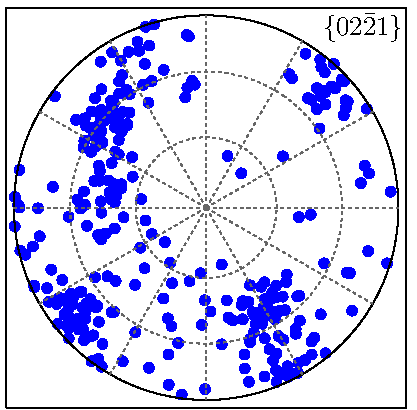
\includegraphics[width=\textwidth]{pic/ebsd1.png}\\
        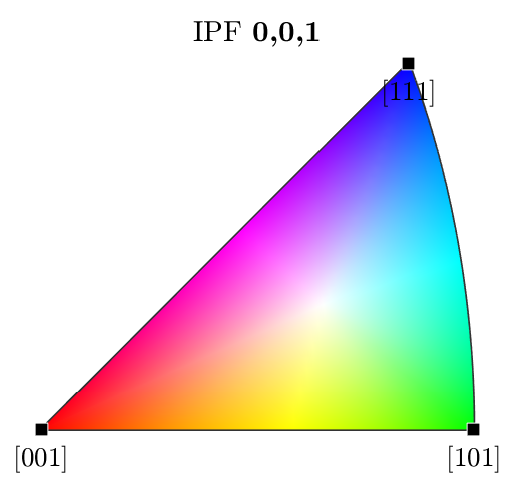
\includegraphics[width=\textwidth]{pic/oM1.png}
      \end{onlyenv}
      \begin{onlyenv}<2>
        \includegraphics[width=\textwidth]{pic/ebsd1Grains.png}\\
        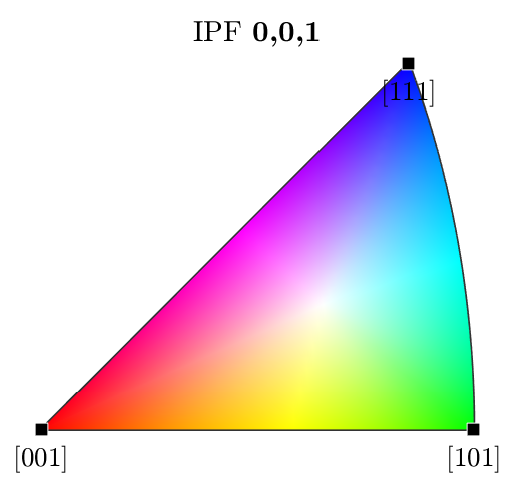
\includegraphics[width=\textwidth]{pic/oM1.png}
      \end{onlyenv}
      \begin{onlyenv}<3>
        \includegraphics[width=\textwidth]{pic/ebsd1mis2meanAngle.png}\\
      \end{onlyenv}
      \begin{onlyenv}<4>
        \includegraphics[width=\textwidth]{pic/ebsd1mis2mean.png}\\
        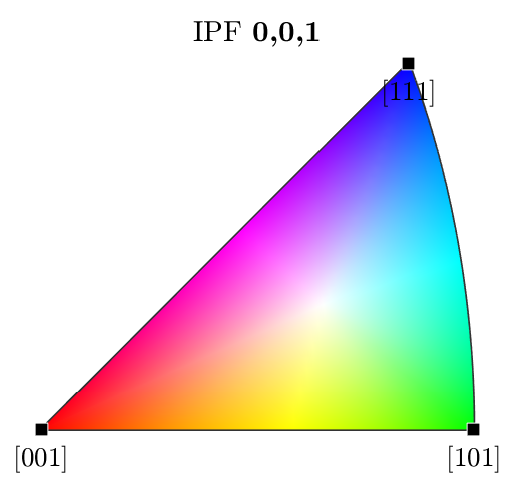
\includegraphics[width=\textwidth]{pic/oM1.png}
      \end{onlyenv}
      \begin{onlyenv}<5>
        \includegraphics[width=\textwidth]{pic/ebsd1mis2meanSharp5.png}\\
        \includegraphics[width=\textwidth]{pic/oMSharp5.png}
      \end{onlyenv}
      \begin{onlyenv}<6>
        \includegraphics[width=\textwidth]{pic/ebsd1mis2meanSharp1.png}\\
        \includegraphics[width=\textwidth]{pic/oMSharp1.png}
      \end{onlyenv}
      \begin{onlyenv}<7>
        \includegraphics[width=\textwidth]{pic/ebsd1mis2meanHalfQuad.png}\\
        \includegraphics[width=\textwidth]{pic/oMSharp1.png}
      \end{onlyenv}
    \end{column}
  \end{columns}

\end{frame}


\begin{frame}[fragile]
  \frametitle{Some Smoothing Techniques}

  \vspace{-0.6cm}
  \begin{overlayarea}{\textwidth}{\textheight}
  \begin{columns}
    \begin{column}{8.3cm}
        \begin{enumerate}
        \item<+-> \structure{Mean Filter:} mean orientation
          of neighbors
        \item<+-> \structure{Median Filter:}  neighboring
          orientation with minimum distance to all other neighboring
          orientations
        \item<+-> \structure{Smoothing Splines:} % Given orientation map $O_{ij}$,
          % determine smoothed map $\tilde O_{ij}$ as solution of the
          % minimization problem
          \begin{equation*}
            \sum_{i,j} \omega(O_{ij},\tilde O_{ij})^{2} + \alpha \nabla
            \tilde O_{ij}^{2} \to \min
          \end{equation*}
        \item<+-> \structure{Half Quadratic Optimization:}
          \begin{equation*}
            \sum_{i,j} \omega(O_{ij},\tilde O_{ij})^{2} + \alpha \left|\nabla
            \tilde O_{ij}\right| \to \min
        \end{equation*}
      \item<+-> \structure{Infimal Convolution:}
          \begin{equation*}
            \sum_{i,j} \omega(O_{ij},\tilde U_{ij} \tilde V_{ij})^{2} + \alpha \left|\nabla
            \tilde U_{ij}\right| + \beta  \left|\triangle
            \tilde V_{ij}\right| \to \min
          \end{equation*}
        \end{enumerate}
    \end{column}
    \begin{column}{3.8cm}
      \begin{onlyenv}<1>
        \includegraphics[width=\textwidth]{pic/ebsd1mis2meanMean.png}\\
        \includegraphics[width=\textwidth]{pic/oMSharp1.png}
      \end{onlyenv}
      \begin{onlyenv}<2>
        \includegraphics[width=\textwidth]{pic/ebsd1mis2meanMedian.png}\\
        \includegraphics[width=\textwidth]{pic/oMSharp1.png}
      \end{onlyenv}
      \begin{onlyenv}<3>
        \includegraphics[width=\textwidth]{pic/ebsd1mis2meanSmooth.png}\\
        \includegraphics[width=\textwidth]{pic/oMSharp1.png}
      \end{onlyenv}
      \begin{onlyenv}<4>
        \includegraphics[width=\textwidth]{pic/ebsd1mis2meanHalfQuad.png}\\
        \includegraphics[width=\textwidth]{pic/oMSharp1.png}
      \end{onlyenv}
      \begin{onlyenv}<5>
        \includegraphics[width=\textwidth]{pic/ebsd1mis2meanInfimal.png}\\
        \includegraphics[width=\textwidth]{pic/oMSharp1.png}
      \end{onlyenv}
    \end{column}
  \end{columns}
    \end{overlayarea}
\end{frame}

\begin{frame}

  \begin{onlyenv}<1>
    \includegraphics[width=\textwidth]{pic/ggRaw.png}

    \begin{center}
      The raw data
    \end{center}
  \end{onlyenv}
  \begin{onlyenv}<2>
    \includegraphics[width=\textwidth]{pic/ggMean.png}

    \begin{center}
      The mean filter
    \end{center}
  \end{onlyenv}

  \begin{onlyenv}<3>
    \includegraphics[width=\textwidth]{pic/ggMedian.png}

    \begin{center}
      The median filter
    \end{center}
  \end{onlyenv}
    \begin{onlyenv}<4>
      \includegraphics[width=\textwidth]{pic/ggSpline.png}

      \begin{center}
        The spline filter
      \end{center}
  \end{onlyenv}
    \begin{onlyenv}<5>
      \includegraphics[width=\textwidth]{pic/gghalfQuad.png}

          \begin{center}
      The halfquadratic filter
    \end{center}
  \end{onlyenv}
    \begin{onlyenv}<6>
      \includegraphics[width=\textwidth]{pic/gginfimal.png}

      \begin{center}
      The infimal convolution filter
    \end{center}
  \end{onlyenv}


\end{frame}



% \begin{frame}
%   \frametitle{Comparison of Smoothing Techniques}

%   \begin{tikzpicture}
%     \begin{axis}[xlabel= x ,width=\textwidth, height=8.5cm,
%       ymin=0,ymax=1,xmax=15,enlargelimits=false,legend pos=north west,%
%       cycle list name=exotic,
%       xtick={0,5,10,15},%
%       xticklabels={0,5,10,15}]
%       \addplot[dotted,mark=o,mark options={scale=.5,solid},thick,black] table[x index=0,y index=1] {matlab/profile.txt};
%       \addplot+[mark=none,thick,blue!80] table[x index=0,y index=2]
%       {matlab/profile.txt};
%       \addplot+[mark=none,thick,green!80!black] table[x index=0,y index=3]
%       {matlab/profile.txt};
%       \addplot+[mark=none,thick,red!80!black] table[x index=0,y index=4]
%       {matlab/profile.txt};
%       \addplot+[mark=none,thick,orange!90!black] table[x index=0,y index=5]
%       {matlab/profile.txt};
%       % \legend{optimal MISE, optimal kernel, Jackson, Dirichlet
%       %  ,  Vallee Poussin, Abel Poisson};
%       \legend{raw data, mean, median, spline, half quadratic};
%     \end{axis}
%   \end{tikzpicture}


% \end{frame}


% \begin{frame}
%   \frametitle{A deformed grain}

%   \begin{overlayarea}{\textwidth}{\textheight}

%     \includegraphics<1->[height=0.45\textheight]{pic/grainRaw.png}
%     \pause
%     \includegraphics<2->[height=0.45\textheight]{pic/grainMis2Mean.png}
%     \pause
%     \includegraphics<3->[height=0.45\textheight]{pic/grainMean.png}

%     \pause
%     \includegraphics<4->[height=0.45\textheight]{pic/grainMedian.png}
%     \pause
%     \includegraphics<5->[height=0.45\textheight]{pic/grainSmooth.png}
%      \pause
%     \includegraphics<6->[height=0.45\textheight]{pic/grainHalfQuad.png}

%   \end{overlayarea}

% \end{frame}


% \begin{frame}
%   \frametitle{Comparison of Smoothing Techniques}

%   \begin{tikzpicture}
%     \begin{axis}[xlabel= x ,width=\textwidth, height=8.5cm,
%       ymin=0,ymax=3,xmax=47,enlargelimits=false,legend pos=north west,%
%       cycle list name=exotic]
%       \addplot[dotted,mark=o,mark options={scale=.5,solid},thick,black] table[x index=0,y index=1] {matlab/profile2.txt};
%       \addplot+[mark=none,thick,blue!80] table[x index=0,y index=2]
%       {matlab/profile2.txt};
%       \addplot+[mark=none,thick,green!80!black] table[x index=0,y index=3]
%       {matlab/profile2.txt};
%       \addplot+[mark=none,thick,red!80!black] table[x index=0,y index=4]
%       {matlab/profile2.txt};
%       \addplot+[mark=none,thick,orange!90!black] table[x index=0,y index=5]
%       {matlab/profile2.txt};
%       % \legend{optimal MISE, optimal kernel, Jackson, Dirichlet
%       %  ,  Vallee Poussin, Abel Poisson};
%       \legend{raw data, mean, median, spline, half quadratic};
%     \end{axis}
%   \end{tikzpicture}


% \end{frame}


\begin{frame}
  \frametitle{A deformed grain}

  \begin{overlayarea}{\textwidth}{\textheight}

    \includegraphics<1->[height=0.45\textheight]{pic/grainRaw.png}
    \;\pause
    \includegraphics<2->[height=0.45\textheight]{pic/grainHalfQuad.png}
    \;\pause
    \includegraphics<3->[height=0.45\textheight]{pic/grainMis2Mean.png}

    \pause

    \includegraphics<4->[height=0.45\textheight]{pic/grainRaw10.png}
    \;\pause
    \includegraphics<5->[height=0.45\textheight]{pic/grainSmooth10.png}
    \;\pause
    \includegraphics<6->[height=0.45\textheight]{pic/grainSmooth10Error.png}

  \end{overlayarea}

\end{frame}



\begin{frame}
  \frametitle{Not Indexed Data}
  \begin{overlayarea}{\textwidth}{\textheight}


    \includegraphics<1->[height=0.45\textheight]{pic/grainRaw50.png}
    \;\pause
    \includegraphics<2->[height=0.45\textheight]{pic/grainSmooth50.png}
    \;\pause
    \includegraphics<3->[height=0.45\textheight]{pic/grainSmooth50Error.png}

    \pause

    \includegraphics<4->[height=0.45\textheight]{pic/grainRaw90.png}
    \;\pause
    \includegraphics<5->[height=0.45\textheight]{pic/grainSmooth90.png}
    \;\pause
    \includegraphics<6->[height=0.45\textheight]{pic/grainSmooth90Error.png}


  \end{overlayarea}

\end{frame}



% \begin{frame}
%   \frametitle{Not Indexed Data}
%   \begin{overlayarea}{\textwidth}{\textheight}

%     \includegraphics<1->[height=0.45\textheight]{pic/grainRaw10.png}
%     \;\pause
%     \includegraphics<2->[height=0.45\textheight]{pic/grainSmooth10.png}
%     \;\pause
%     \includegraphics<3->[height=0.45\textheight]{pic/grainSmooth10Error.png}

%     \pause
%     \includegraphics<4->[height=0.45\textheight]{pic/grainRaw50.png}
%     \;\pause
%     \includegraphics<5->[height=0.45\textheight]{pic/grainSmooth50.png}
%     \;\pause
%     \includegraphics<6->[height=0.45\textheight]{pic/grainSmooth50Error.png}

%   \end{overlayarea}

% \end{frame}

% \begin{frame}
%   \frametitle{Not Indexed Data}

%   \begin{overlayarea}{\textwidth}{\textheight}
%     \includegraphics<1->[height=0.45\textheight]{pic/grainRaw90.png}
%     \;
%     \pause
%     \includegraphics<2->[height=0.45\textheight]{pic/grainSmooth90.png}
%     \;
%     \pause
%     \includegraphics<3->[height=0.45\textheight]{pic/grainSmooth90Error.png}

%     \pause
%     \includegraphics<4->[height=0.45\textheight]{pic/grainRaw90.png}
%     \;
%     \pause
%     \includegraphics<5->[height=0.45\textheight]{pic/grainHalfQuad90.png}
%     \;
%     \pause
%     \includegraphics<6->[height=0.45\textheight]{pic/grainHalfQuad90Error.png}

%   \end{overlayarea}
% \end{frame}


\begin{frame}[fragile]
  \frametitle{Grains from partly not indexed data}
  \begin{overlayarea}{\textwidth}{\textheight}
    \includegraphics<1>[width=\textwidth]{pic/ebsdGrainRaw.png}
    \includegraphics<2>[width=\textwidth]{pic/ebsdGrain1.png}
    \includegraphics<3>[width=\textwidth]{pic/ebsdGrain2.png}
    \includegraphics<4>[width=\textwidth]{pic/ebsdGrain5.png}
    \includegraphics<5>[width=\textwidth]{pic/ebsdGrain6.png}
    % \includegraphics<6>[width=\textwidth]{pic/emptyGrainIndex.png}
    % \includegraphics<7>[width=\textwidth]{pic/ebsdGrain3.png}
    \begin{onlyenv}<2>
\begin{lstlisting}[style=input]
grains = calcGrains(ebsd)
\end{lstlisting}
    \end{onlyenv}
    \begin{onlyenv}<3>
      \vspace{-0.5cm}
\begin{lstlisting}[style=input]
grains = calcGrains(ebsd('indexed'))
\end{lstlisting}
    \end{onlyenv}
        \begin{onlyenv}<4>
      \vspace{-0.5cm}
\begin{lstlisting}[style=input]
ebsd = smooth(ebsd,F,grains,'fill')
\end{lstlisting}
    \end{onlyenv}
            \begin{onlyenv}<5>
      \vspace{-0.5cm}
\begin{lstlisting}[style=input]
plot(ebsd,ebsd.mis2mean)
\end{lstlisting}
    \end{onlyenv}
  \end{overlayarea}

\end{frame}

\begin{frame}
\frametitle{A synthetic example}

\begin{overlayarea}{\textwidth}{8cm}

  \hspace{2.5cm}
  \includegraphics[height=1.75cm]{pic/sim.png}

  \pause
  \medskip

  \hspace{2.5cm}
  \includegraphics<2->[height=1.75cm]{pic/simNoise.png}


  \pause
  \medskip

  \hspace{2.5cm}
  \includegraphics<3->[height=2cm]{pic/kamSimNoiseFree}


  \pause
  \medskip

  \hspace{2.5cm}
  \includegraphics<4>[height=2cm]{pic/kamSimNoise}

\end{overlayarea}
\end{frame}


\begin{frame}
  \frametitle{KAM}
    \centering
    \begin{tikzpicture}
    \begin{axis}[width=\textwidth,height=7cm, ymin=-0.1,ymax=2.5,xmax=100,enlargelimits=false,
      cycle list name=exotic,
      legend columns = 5,
      legend style={at={(0.5,-0.2)},anchor=north}]
      \addplot+[mark=none, very thick] table[x index=0,y index=1]{pic/kamSim.txt};
      \addplot+[mark=none, thick] table[x index=0,y index=2]{pic/kamSim.txt};
      \addplot+[mark=none, thick] table[x index=0,y index=3]{pic/kamSim.txt};
      \addplot+[mark=none, thick] table[x index=0,y index=4]{pic/kamSim.txt};
      \addplot+[mark=none, thick] table[x index=0,y index=5]{pic/kamSim.txt};
      \legend{no noise, $\delta = 0.25^{\circ}$, $\delta = 0.5^{\circ}$, $\delta = 0.75^{\circ}$, $\delta = 1^{\circ}$}
    \end{axis}
  \end{tikzpicture}
\end{frame}


\begin{frame}[fragile]
  \frametitle{Basic Denoising Techniques}

  \begin{overlayarea}{\textwidth}{8cm}
    \begin{center}
      \begin{tikzpicture}
        \begin{axis}[width=0.43\textwidth,height=4.5cm,
          ymin=-20,ymax=20,xmax=100,enlargelimits=false, cycle list
          name=exotic,legend pos=south west,hide x axis, hide y axis, legend
          style={cells={anchor=west}}]
          \addplot+[mark=none] table[x index=0,y index=1]
          {pic/meanSimSec.txt}; \addplot graphics
          [ymin=-20,ymax=-1,xmin=0,xmax=100]{pic/meanSim1.png};
        \end{axis}
      \end{tikzpicture}
      \begin{tikzpicture}
        \begin{axis}[width=0.43\textwidth,height=4.5cm,
          ymin=-20,ymax=20,xmax=100,enlargelimits=false, cycle list
          name=exotic,legend pos=south west,hide x axis, hide y axis, legend
          style={cells={anchor=west}}]
          \addplot+[mark=none] table[x index=0,y index=2]
          {pic/meanSimSec.txt}; \addplot graphics
          [ymin=-20,ymax=-1,xmin=0,xmax=100]{pic/meanSim2.png};
        \end{axis}
      \end{tikzpicture}
      \begin{tikzpicture}
        \begin{axis}[width=0.43\textwidth,height=4.5cm,
          ymin=-20,ymax=20,xmax=100,enlargelimits=false, cycle list
          name=exotic,legend pos=south west,hide x axis, hide y axis, legend
          style={cells={anchor=west}}]
          \addplot+[mark=none] table[x index=0,y index=3]
          {pic/meanSimSec.txt}; \addplot graphics
          [ymin=-20,ymax=-1,xmin=0,xmax=100]{pic/meanSim3.png};
        \end{axis}
      \end{tikzpicture}
    \end{center}
    \vspace{-0.3cm}
    \centering{noisy data, mean filter: first and second neighbor}

    \pause \medskip

    \begin{onlyenv}<2>
      \begin{center}
        \begin{tikzpicture}
          \begin{axis}[width=0.43\textwidth,height=4.5cm,
            ymin=-20,ymax=20,xmax=100,enlargelimits=false, cycle list
            name=exotic,legend pos=south west,hide x axis, hide y axis, legend
            style={cells={anchor=west}}]
            \addplot+[mark=none] table[x index=0,y index=1]
            {pic/medianSimSec.txt}; \addplot graphics
            [ymin=-20,ymax=-1,xmin=0,xmax=100]{pic/medianSim1.png};
          \end{axis}
        \end{tikzpicture}
        \begin{tikzpicture}
          \begin{axis}[width=0.43\textwidth,height=4.5cm,
            ymin=-20,ymax=20,xmax=100,enlargelimits=false, cycle list
            name=exotic,legend pos=south west,hide x axis, hide y axis, legend
            style={cells={anchor=west}}]
            \addplot+[mark=none] table[x index=0,y index=2]
            {pic/medianSimSec.txt}; \addplot graphics
            [ymin=-20,ymax=-1,xmin=0,xmax=100]{pic/medianSim2.png};
          \end{axis}
        \end{tikzpicture}
        \begin{tikzpicture}
          \begin{axis}[width=0.43\textwidth,height=4.5cm,
            ymin=-20,ymax=20,xmax=100,enlargelimits=false, cycle list
            name=exotic,legend pos=south west,hide x axis, hide y axis, legend
            style={cells={anchor=west}}]
            \addplot+[mark=none] table[x index=0,y index=3]
            {pic/medianSimSec.txt}; \addplot graphics
            [ymin=-20,ymax=-1,xmin=0,xmax=100]{pic/medianSim3.png};
          \end{axis}
        \end{tikzpicture}
      \end{center}
      \vspace{-0.3cm}
      \centering{median filter: first, third, and fifth neighbor}
    \end{onlyenv}
  \end{overlayarea}
\end{frame}

\begin{frame}

\frametitle{Advanced Denoising Techniques}

  \begin{overlayarea}{\textwidth}{8.5cm}
    \begin{center}
      \begin{tikzpicture}
        \begin{axis}[width=0.43\textwidth,height=4.5cm,
          ymin=-20,ymax=20,xmax=100,enlargelimits=false, cycle list
          name=exotic,legend pos=south west,hide x axis, hide y axis, legend
          style={cells={anchor=west}}]
          \addplot+[mark=none] table[x index=0,y index=2]
          {pic/splineSimSec.txt}; \addplot graphics
          [ymin=-20,ymax=-1,xmin=0,xmax=100]{pic/splineSim2.png};
        \end{axis}
      \end{tikzpicture}
      \begin{tikzpicture}
        \begin{axis}[width=0.43\textwidth,height=4.5cm,
          ymin=-20,ymax=20,xmax=100,enlargelimits=false, cycle list
          name=exotic,legend pos=south west,hide x axis, hide y axis, legend
          style={cells={anchor=west}}]
          \addplot+[mark=none] table[x index=0,y index=1]
          {pic/splineSimSec.txt}; \addplot graphics
          [ymin=-20,ymax=-1,xmin=0,xmax=100]{pic/splineSim1.png};
        \end{axis}
      \end{tikzpicture}
      \begin{tikzpicture}
        \begin{axis}[width=0.43\textwidth,height=4.5cm,
          ymin=-20,ymax=20,xmax=100,enlargelimits=false, cycle list
          name=exotic,legend pos=south west,hide x axis, hide y axis, legend
          style={cells={anchor=west}}]
          \addplot+[mark=none] table[x index=0,y index=3]
          {pic/splineSimSec.txt}; \addplot graphics
          [ymin=-20,ymax=-1,xmin=0,xmax=100]{pic/splineSim3.png};
        \end{axis}
      \end{tikzpicture}
    \end{center}
    \vspace{-0.3cm}
    \centering{smoothing spline filter with $\alpha=0.1$ , $\alpha=0.58$, and
      $\alpha=5$}

    \pause

    \begin{onlyenv}<2>
      \begin{center}
        \begin{tikzpicture}
          \begin{axis}[width=0.43\textwidth,height=4.5cm,
            ymin=-20,ymax=20,xmax=100,enlargelimits=false, cycle list
            name=exotic,legend pos=south west,hide x axis, hide y axis, legend
            style={cells={anchor=west}}]
            \addplot+[mark=none] table[x index=0,y index=1]
            {pic/halfquadSimSec.txt}; \addplot graphics
            [ymin=-20,ymax=-1,xmin=0,xmax=100]{pic/halfquadSim1.png};
          \end{axis}
        \end{tikzpicture}
        \begin{tikzpicture}
          \begin{axis}[width=0.43\textwidth,height=4.5cm,
            ymin=-20,ymax=20,xmax=100,enlargelimits=false, cycle list
            name=exotic,legend pos=south west,hide x axis, hide y axis, legend
            style={cells={anchor=west}}]
            \addplot+[mark=none] table[x index=0,y index=2]
            {pic/halfquadSimSec.txt}; \addplot graphics
            [ymin=-20,ymax=-1,xmin=0,xmax=100]{pic/halfquadSim2.png};
          \end{axis}
        \end{tikzpicture}
        \begin{tikzpicture}
          \begin{axis}[width=0.43\textwidth,height=4.5cm,
            ymin=-20,ymax=20,xmax=100,enlargelimits=false, cycle list
            name=exotic,legend pos=south west,hide x axis, hide y axis, legend
            style={cells={anchor=west}}]
            \addplot+[mark=none] table[x index=0,y index=3]
            {pic/halfquadSimSec.txt}; \addplot graphics
            [ymin=-20,ymax=-1,xmin=0,xmax=100]{pic/halfquadSim3.png};
          \end{axis}
        \end{tikzpicture}
      \end{center}
      \vspace{-0.3cm}
      \centering{half quadratic filter with $\alpha=0.025$, $\alpha=0.1$, and
        $\alpha=0.5$}
    \end{onlyenv}
  \end{overlayarea}

\end{frame}

\begin{frame}[fragile]
\frametitle{Advanced Denoising Techniques}

\begin{center}
  \begin{tikzpicture}
    \begin{axis}[width=0.43\textwidth,height=4.5cm,
      ymin=-20,ymax=20,xmax=100,enlargelimits=false, cycle list
      name=exotic,legend pos=south west,hide x axis, hide y axis, legend
      style={cells={anchor=west}}]
      \addplot+[mark=none] table[x index=0,y index=1]
      {pic/infimalSimSec.txt}; \addplot graphics
      [ymin=-20,ymax=-1,xmin=0,xmax=100]{pic/infimalSim1.png};
    \end{axis}
  \end{tikzpicture}
  \begin{tikzpicture}
    \begin{axis}[width=0.43\textwidth,height=4.5cm,
      ymin=-20,ymax=20,xmax=100,enlargelimits=false, cycle list
      name=exotic,legend pos=south west,hide x axis, hide y axis, legend
      style={cells={anchor=west}}]
      \addplot+[mark=none] table[x index=0,y index=2]
      {pic/infimalSimSec.txt}; \addplot graphics
      [ymin=-20,ymax=-1,xmin=0,xmax=100]{pic/infimalSim2.png};
    \end{axis}
  \end{tikzpicture}
  \begin{tikzpicture}
    \begin{axis}[width=0.43\textwidth,height=4.5cm,
      ymin=-20,ymax=20,xmax=100,enlargelimits=false, cycle list
      name=exotic,legend pos=south west,hide x axis, hide y axis, legend
      style={cells={anchor=west}}]
      \addplot+[mark=none] table[x index=0,y index=3]
      {pic/infimalSimSec.txt}; \addplot graphics
      [ymin=-20,ymax=-1,xmin=0,xmax=100]{pic/infimalSim3.png};
    \end{axis}
  \end{tikzpicture}
\end{center}
\vspace{-0.3cm}
\centering{infimal convolution spline filter with $\alpha=0.01$ , $\alpha=0.05$, and
  $\alpha=1$}
\end{frame}

  \begin{frame}
  \frametitle{KAM of Denoised Data}
      \begin{tikzpicture}
    \begin{axis}[width=\textwidth,height=7cm, ymin=0,ymax=2.5,xmax=100,enlargelimits=false,
      cycle list name=exotic,legend pos=south west,
      legend columns = 5,
      legend style={at={(0.5,-0.2)},anchor=north}]
      \addplot+[mark=none, very thick] table[x index=0,y index=1]{pic/kamSim.txt};
      \addplot+[mark=none, very thick] table[x index=0,y index=1]{pic/kamSimSec.txt};
      \addplot+[mark=none, thick] table[x index=0,y index=2]{pic/kamSimSec.txt};
      \addplot+[mark=none, thick] table[x index=0,y index=3]{pic/kamSimSec.txt};
      \addplot+[mark=none, thick] table[x index=0,y index=4]{pic/kamSimSec.txt};
      \addplot+[mark=none, thick] table[x index=0,y index=5]{pic/kamSimSec.txt};
      \addplot+[mark=none, thick] table[x index=0,y index=6]{pic/kamSimSec.txt};

      \legend{no noise, no de noising, $\alpha = 0.01$, $\alpha = 0.04$,
        $\alpha = 0.1$, $\alpha = 0.4$,
        $\alpha = 1$}
    \end{axis}
  \end{tikzpicture}

\end{frame}


\end{document}


%%% Local Variables:
%%% mode: latex
%%% TeX-master: t
%%% End:
